\documentclass[border=6pt]{standalone}
\usepackage[fontset=fandol]{ctex}
\usepackage{amsmath,amssymb,tikz}
\usetikzlibrary{arrows.meta,calc,decorations.pathmorphing}
\begin{document}

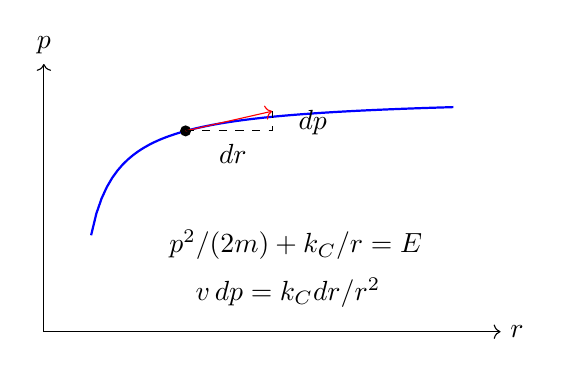
\begin{tikzpicture}
\draw[->](0,0)--(5.8,0)node[right]{$r$};
\draw[->](0,0)--(0,3.4)node[above]{$p$};
\draw[blue,thick]plot[domain=.6:5.2,samples=70](\x,{3*sqrt(1-.5/\x)});
\fill(1.8,2.55)circle(2pt);
\draw[->,red](1.8,2.55)--(2.9,2.8);
\draw[dashed](1.8,2.55)--(2.9,2.55)--(2.9,2.8);
\node[below]at(2.4,2.5){$dr$};\node[right=6pt]at(2.9,2.65){$dp$};
\node at(3.2,1.1){$p^2/(2m)+k_C/r=E$};
\node at(3.1,.5){$v\,dp=k_Cdr/r^2$};
\end{tikzpicture}

\end{document}
